% VLSI LAB REPORT STRUCTURE TEMPLATE
% CREATED BY ISTIAK ALAM (CSE-20)
\documentclass[12pt,a4paper]{report}
\usepackage[utf8]{inputenc}
\usepackage[T1]{fontenc}
\usepackage{fontspec}
\setmainfont{Times New Roman}
\newfontfamily\hackfont{Hack}
\usepackage{titlesec}
\usepackage{fancyhdr}
\usepackage{listings}
\usepackage{xcolor}
\usepackage{graphicx}
\usepackage{longtable}
\usepackage{caption}
\usepackage{hyperref}
\usepackage{setspace}
\usepackage{geometry}
\geometry{a4paper, margin=1in}
\hypersetup{colorlinks=true, linkcolor=blue, urlcolor=blue}
\renewcommand{\contentsname}{Table of Contents}
\titleformat{\chapter}
  {\centering\Huge\bfseries}  % centering Chapter Name
  {Lab \thechapter}               
  {1em}
  {} 


\begin{document}

\begin{titlepage}					% Cover Start
\begin{center}
    
\includegraphics[width=0.35\textwidth]{logo.png} \\
    \vspace{0.5cm}
    \textbf{\Huge \textcolor{cyan}{NOTRE DAME} \textcolor{cyan}{UNIVERSITY}} \\
    \vspace{0.5cm}
    \textbf{\Huge \textcolor{orange}{BANGLADESH}} \\
    
    \vspace{0.9cm}
    \textbf{\Huge \underline{VLSI Design Lab Report}} \\
    
    \vspace{1.5em}
    \begin{flushleft}
    	\textbf{\Large Course Code: CSE-4218} \\
		\vspace{0.3cm}        
        \textbf{\Large Course Title: VLSI Design Lab} \\
        \vspace{0.3cm}
        \textbf{\Large Experiment Name: All the experiments} \\        
    \end{flushleft}
    
    \vspace{1em}
    \begin{flushleft}
        \textbf{\Huge \textcolor{blue}{Submitted by:}} \\
        \vspace{0.3cm}
        \textbf{\Large Name: } \\
        \vspace{0.3cm}
        \textbf{\Large ID: } \\
		\vspace{0.3cm}        
        \textbf{\Large Batch: CSE-20} \\
        \vspace{0.5cm}
        \textbf{\Large Submission Date: }{\Large \textbf{\today}\par}
    \end{flushleft}
    \vfill
    \begin{flushleft}
        \textbf{\Huge \textcolor{blue}{Submitted to:}} \\
        \vspace{0.3cm}
        \textbf{\Large Nafisa Tabassum,} \\
        \vspace{0.3cm}
        \textbf{\Large Lecturer, Dept of CSE} \\
        \vspace{0.3cm}
        \textbf{\Large Notre Dame University Bangladesh}
    \end{flushleft}
\end{center}
\end{titlepage}						% Cover End

% Table of Contents
\tableofcontents
\thispagestyle{empty}
\clearpage
\pagenumbering{arabic}

% Header Sections 
\pagestyle{fancy}
\fancyhf{} 							% Header Middle
\rhead{VLSI Design Lab}
\rfoot{\thepage}

\chapter*{\center Abstract}
\addcontentsline{toc}{chapter}{Abstract}
\thispagestyle{empty}

<Write Abstract here>


\chapter*{\center Software Information}
\addcontentsline{toc}{chapter}{Software Information}
<Write Software information here>

\newpage
\chapter{CMOS Logic Gate in DSCH2}
\lhead{Lab-01: CMOS Logic Gate in DSCH2}

\section{Inverter / NOT Gate}
A NOT gate, also known as an inverter, produces the complement of its input.



\subsection*{Schematic Image}
\begin{figure}[h!]
    \centering
    \includegraphics[width=0.6\textwidth]{Lab-01/1in-inverter.png}
    \caption{Schematic of the 1-input Inverter}
\end{figure}

\subsection*{Truth Table}
\begin{center}
\begin{tabular}{|c|c|}
\hline
A & Y \\ \hline
0 & 1 \\
1 & 0 \\ \hline
\end{tabular}
\end{center}

\subsection*{Observation}
From the truth table and simulation results, it is observed that the output of the inverter is always the logical complement of the input. When the input \(A = 0\), the output \(Y\) becomes logic HIGH (1), and when the input \(A = 1\), the output \(Y\) becomes logic LOW (0). This confirms that the inverter correctly performs logical inversion for all possible input conditions.





\section{2-input NAND}
A 2-input NAND gate is a universal logic gate that produces a logic LOW output only when both inputs are logic HIGH. For all other input combinations, the output remains logic HIGH. Due to its universality, complex digital circuits can be implemented using only NAND gates.

\subsection*{Schematic Image}
\begin{figure}[h!]
    \centering
    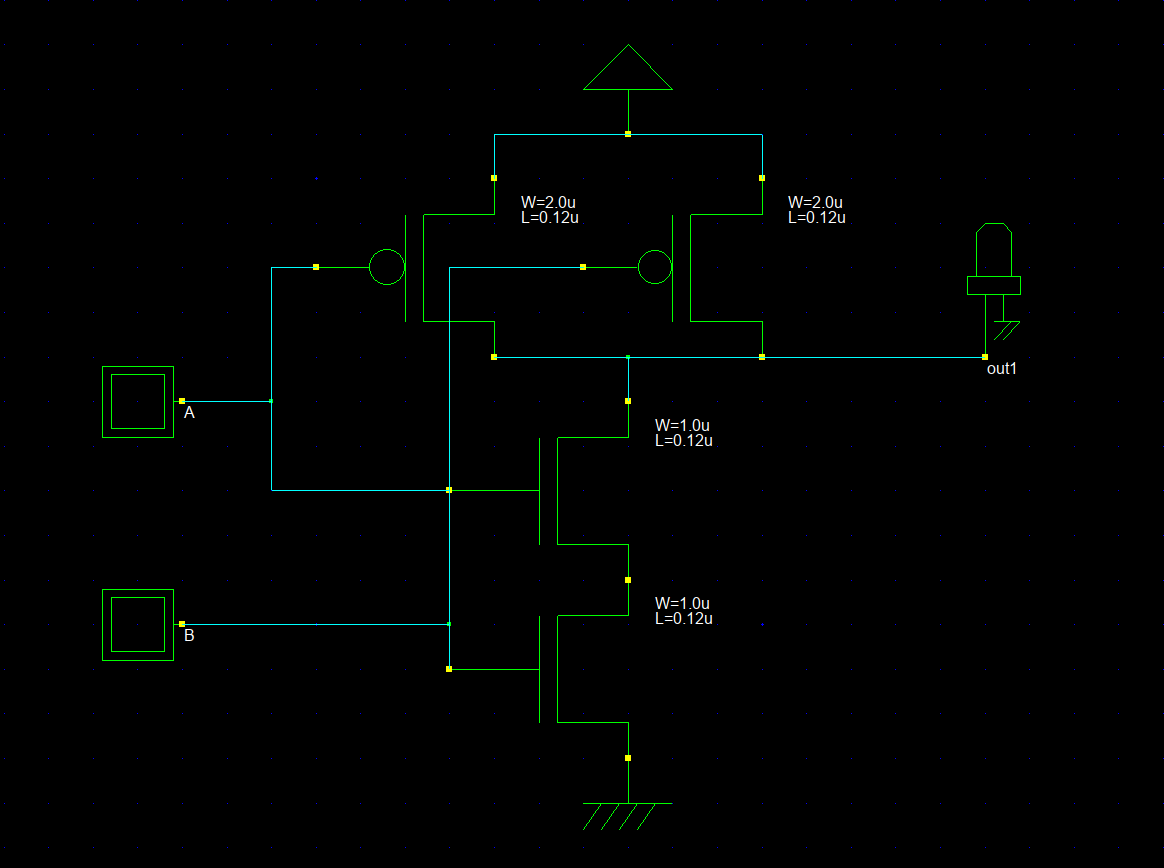
\includegraphics[width=0.8\textwidth]{Lab-01/2in-NAND.png}
    \caption{Schematic of the 2-input NAND}
\end{figure}

\subsection*{Truth Table}
\begin{center}
\begin{tabular}{|c|c|c|}
\hline
A & B & Y \\ \hline
0 & 0 & 1 \\
0 & 1 & 1 \\
1 & 0 & 1 \\
1 & 1 & 0 \\ \hline
\end{tabular}
\end{center}

\subsection*{Observation}
From the simulation results in DSCH2, it was observed that the output of the 2-input NAND gate remains at logic HIGH for all input combinations except when both inputs A and B are logic HIGH. When either input is logic LOW, the output stays HIGH. The output transitions to logic LOW only for the input condition A = 1 and B = 1. These observations are fully consistent with the theoretical truth table of a 2-input NAND gate, confirming correct logical operation of the designed schematic.




\section{3-input NAND}
A 3-input NAND gate outputs a logic LOW only when all three inputs are logic HIGH. For any other input combination, the output remains logic HIGH.

\subsection*{Schematic Image}
\begin{figure}[h!]
    \centering
    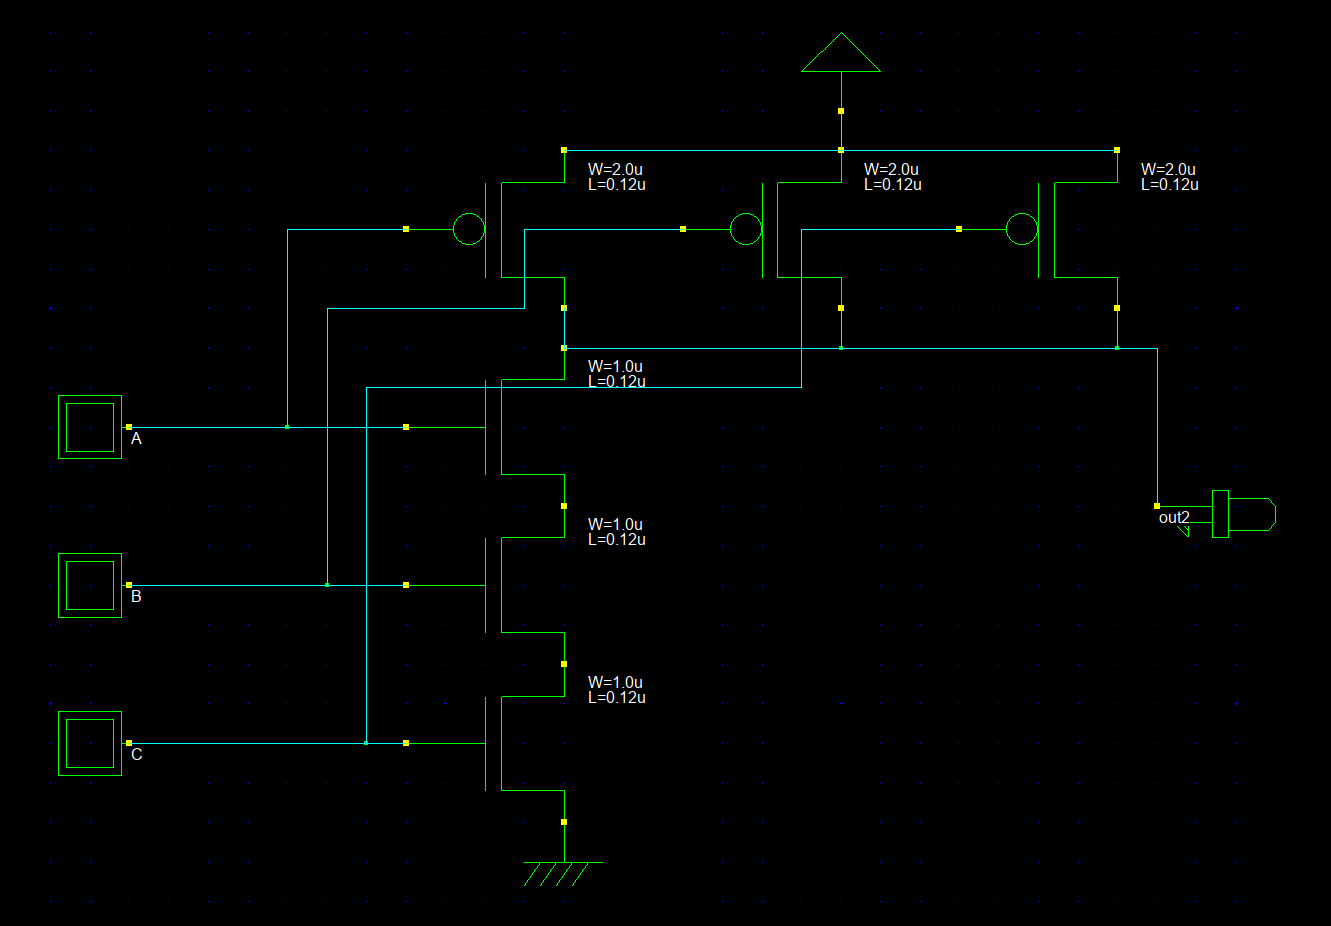
\includegraphics[width=0.7\textwidth]{Lab-01/3in-NAND.png}
    \caption{Schematic of the 3-input NAND}
\end{figure}

\subsection*{Truth Table}
\begin{center}
\begin{tabular}{|c|c|c|c|}
\hline
A & B & C & Y \\ \hline
0 & 0 & 0 & 1 \\
0 & 0 & 1 & 1 \\
0 & 1 & 0 & 1 \\
0 & 1 & 1 & 1 \\
1 & 0 & 0 & 1 \\
1 & 0 & 1 & 1 \\
1 & 1 & 0 & 1 \\
1 & 1 & 1 & 0 \\ \hline
\end{tabular}
\end{center}

\subsection*{Observation}
From the truth table and simulation results, it was observed that the output of the 3-input NAND gate remains at logic HIGH for all input combinations except when all three inputs (A, B, and C) are simultaneously at logic HIGH. In the case where A = 1, B = 1, and C = 1, the output transitions to logic LOW. This behavior confirms that the gate performs the logical negation of the AND operation for three inputs. The observed output values from the DSCH2 simulation precisely matched the theoretical truth table, indicating correct functionality of the 3-input NAND gate.


% ---------------------------------------------------


\section{2-input NOR}
A 2-input NOR gate produces a logic HIGH output only when both inputs are logic LOW. For all other input combinations, the output is logic LOW. NOR gates are also universal gates in digital logic design.

\subsection*{Schematic Image}
\begin{figure}[h!]
    \centering
    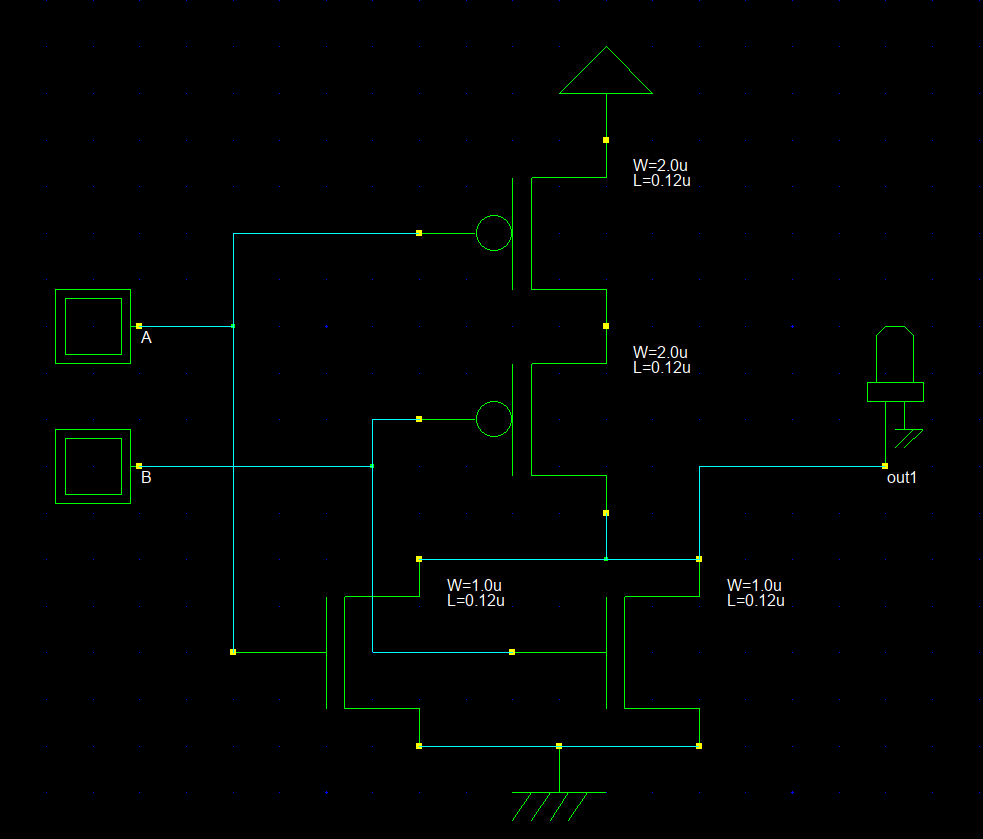
\includegraphics[width=0.8\textwidth]{Lab-01/2in-NOR.png}
    \caption{Schematic of the 2-input NOR}
\end{figure}

\subsection*{Truth Table}
\begin{center}
\begin{tabular}{|c|c|c|}
\hline
A & B & Y \\ \hline
0 & 0 & 1 \\
0 & 1 & 0 \\
1 & 0 & 0 \\
1 & 1 & 0 \\ \hline
\end{tabular}
\end{center}

\subsection*{Observation}
From the truth table and simulation results, it is observed that the output of the 2-input NOR gate remains at logic HIGH only when both inputs A and B are at logic LOW. For all other input combinations where at least one input is logic HIGH, the output transitions to logic LOW. This behavior confirms that the circuit performs the logical NOR operation correctly, as verified through DSCH2 simulation.


% ---------------------------------------------------


\section{3-input NOR}

\subsection*{Schematic Image}
\begin{figure}[h!]
    \centering
    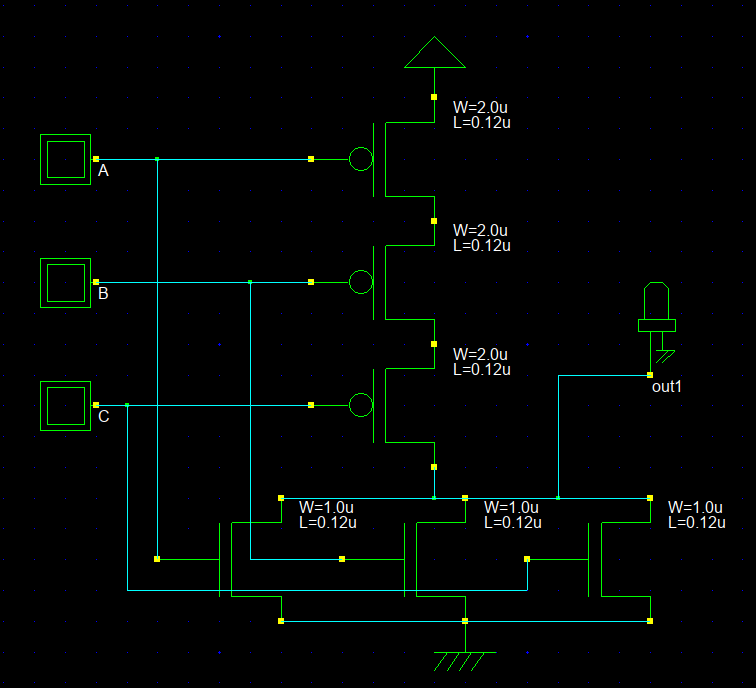
\includegraphics[width=0.65\textwidth]{Lab-01/3in-NOR.png}
    \caption{Schematic of the 3-input NOR}
\end{figure}

\subsection*{Truth Table}
\begin{center}
\begin{tabular}{|c|c|c|c|}
\hline
A & B & C & Y \\ \hline
0 & 0 & 0 & 1 \\
0 & 0 & 1 & 0 \\
0 & 1 & 0 & 0 \\
0 & 1 & 1 & 0 \\
1 & 0 & 0 & 0 \\
1 & 0 & 1 & 0 \\
1 & 1 & 0 & 0 \\
1 & 1 & 1 & 0 \\ \hline
\end{tabular}
\end{center}

\subsection*{Observation}
From the simulation results, it is observed that the output of the 3-input NOR gate becomes logic HIGH only when all three inputs (A, B, and C) are at logic LOW. For any input combination where at least one input is HIGH, the output remains logic LOW. This behavior is consistent with the truth table of the 3-input NOR gate. The DSCH2 simulation output accurately reflects the expected NOR operation, confirming the correctness of the schematic design.


% ---------------------------------------------------


\section{AND Gate}
An AND gate outputs logic HIGH only when all inputs are HIGH.

\subsection*{Schematic Image}
\begin{figure}[h!]
    \centering
    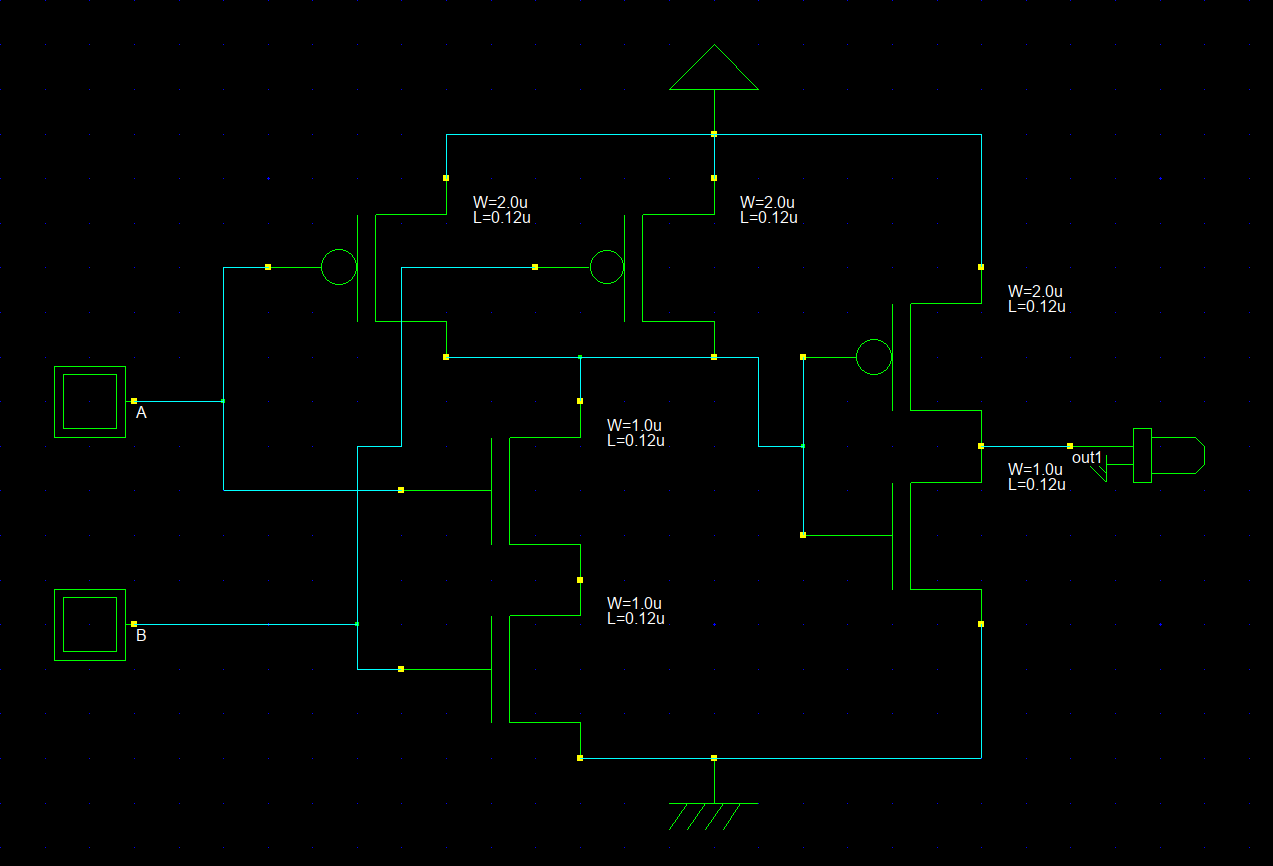
\includegraphics[width=1\textwidth]{Lab-01/2in-AND.png}
    \caption{Schematic of the AND Gate}
\end{figure}

\subsection*{Truth Table}
\begin{center}
\begin{tabular}{|c|c|c|}
\hline
A & B & Y \\ \hline
0 & 0 & 0 \\
0 & 1 & 0 \\
1 & 0 & 0 \\
1 & 1 & 1 \\ \hline
\end{tabular}
\end{center}

\subsection*{Observation}
From the simulation results of the 2-input AND gate in DSCH2, it was observed that the output remains at logic LOW when any one or both of the inputs are at logic LOW. The output transitions to logic HIGH only when both inputs A and B are simultaneously at logic HIGH. This behavior is consistent with the truth table of an AND gate, confirming that the implemented schematic operates correctly.


% ---------------------------------------------------


\section{OR Gate}
An OR gate produces logic HIGH when at least one input is HIGH.

\subsection*{Schematic Image}
\begin{figure}[h!]
    \centering
    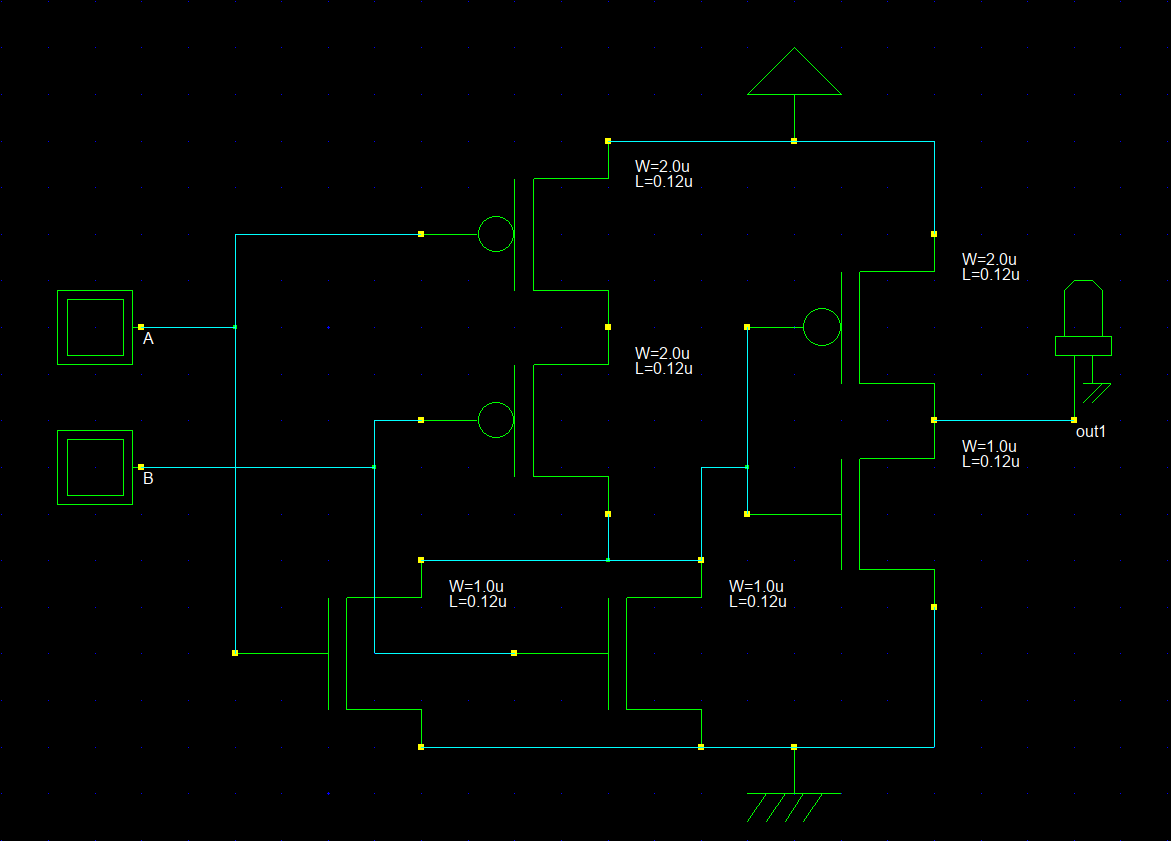
\includegraphics[width=0.9\textwidth]{Lab-01/2in-OR.png}
    \caption{Schematic of the OR Gate}
\end{figure}

\subsection*{Truth Table}
\begin{center}
\begin{tabular}{|c|c|c|}
\hline
A & B & Y \\ \hline
0 & 0 & 0 \\
0 & 1 & 1 \\
1 & 0 & 1 \\
1 & 1 & 1 \\ \hline
\end{tabular}
\end{center}

\subsection*{Observation}
From the simulation results obtained in DSCH2, it was observed that the output of the 2-input OR gate becomes logic HIGH whenever at least one of the inputs is at logic HIGH. When both inputs A and B are at logic LOW, the output remains logic LOW. The simulation output exactly follows the theoretical truth table of the OR gate, confirming that the gate correctly performs the logical OR operation.



% ---------------------------------------------------


\section{XOR Gate}
An XOR gate outputs logic HIGH when the inputs are different.

\subsection*{Schematic Image}
\begin{figure}[h!]
    \centering
    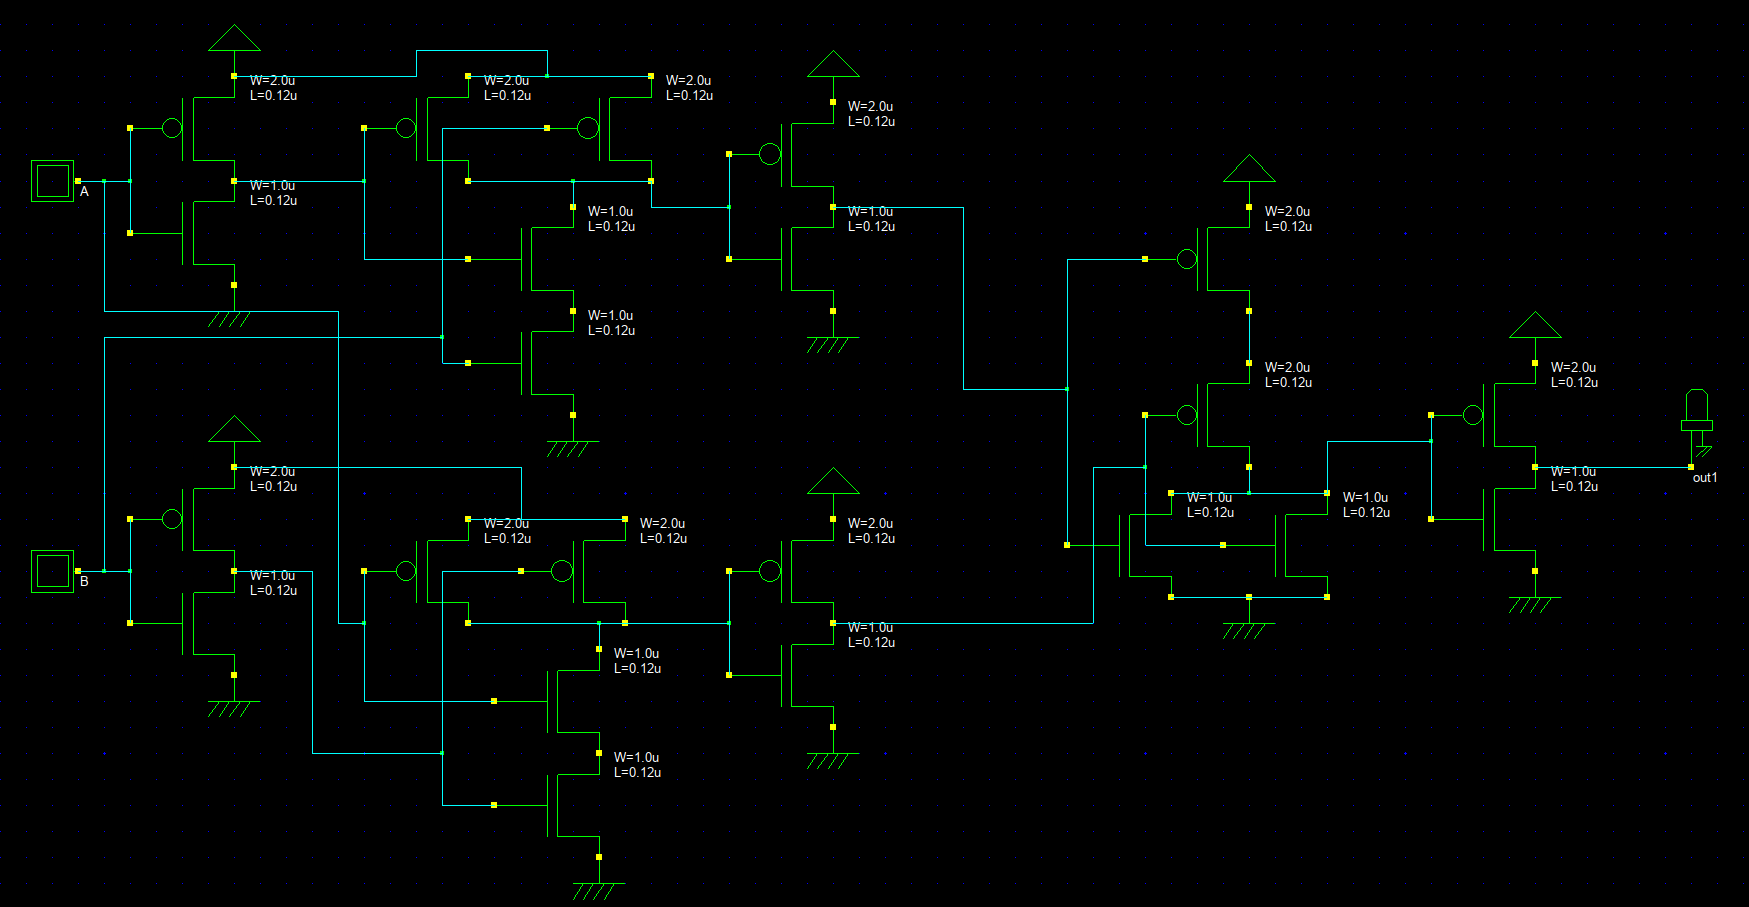
\includegraphics[width=1\textwidth]{Lab-01/2in-XOR.png}
    \caption{Schematic of the XOR Gate}
\end{figure}

\subsection*{Truth Table}
\begin{center}
\begin{tabular}{|c|c|c|}
\hline
A & B & Y \\ \hline
0 & 0 & 0 \\
0 & 1 & 1 \\
1 & 0 & 1 \\
1 & 1 & 0 \\ \hline
\end{tabular}
\end{center}

\subsection*{Observation}
From the simulation results of the 2-input XOR gate in DSCH2, it was observed that the output remains logic LOW when both inputs are at the same logic level, i.e., when both inputs are LOW (0,0) or both inputs are HIGH (1,1). The output becomes logic HIGH when the inputs are different, i.e., for input combinations (0,1) and (1,0). These observations exactly match the theoretical truth table of the XOR gate, confirming that the circuit correctly performs the exclusive-OR operation.





\chapter{Implementing Sequential Circuit}
\lhead{Lab-02: Implementing Sequential Circuit}
\section*{Introduction}
The objective of this laboratory experiment is to implement given Boolean expressions using CMOS logic and verify their functional correctness through schematic design and timing simulation. The circuits were designed using the DSCH2 schematic editor, following standard CMOS pull-up and pull-down network principles. Truth tables and timing diagrams were analyzed to validate logical behavior.


\section*{Objective}
The objectives of this VLSI-Lab experiment are as follows:
\begin{itemize}
    \item To implement given Boolean expressions using CMOS logic design methodology.
    \item To design schematic-level CMOS circuits using the DSCH2 tool.
    \item To verify the logical correctness of the implemented circuits using truth tables.
    \item To analyze timing diagrams to observe signal transitions and propagation behavior.
    \item To develop a clear understanding of CMOS pull-up and pull-down network operation.
\end{itemize}

\section{Function 1: $(ABC + D)'$}

\subsection*{Boolean Function}
\[
Y = (ABC + D)'
\]

\subsection*{Truth Table}
\begin{center}
\begin{tabular}{|c|c|c|c|c|}
\hline 
A & B & C & D & Y \\ \hline
0 & 0 & 0 & 0 & 1 \\
0 & 0 & 1 & 0 & 1 \\
0 & 1 & 0 & 0 & 1 \\
0 & 1 & 1 & 0 & 1 \\
1 & 1 & 1 & 0 & 0 \\
X & X & X & 1 & 0 \\ \hline
\end{tabular}
\end{center}

\subsection*{Schematic Image}
\begin{figure}[!h]
\centering
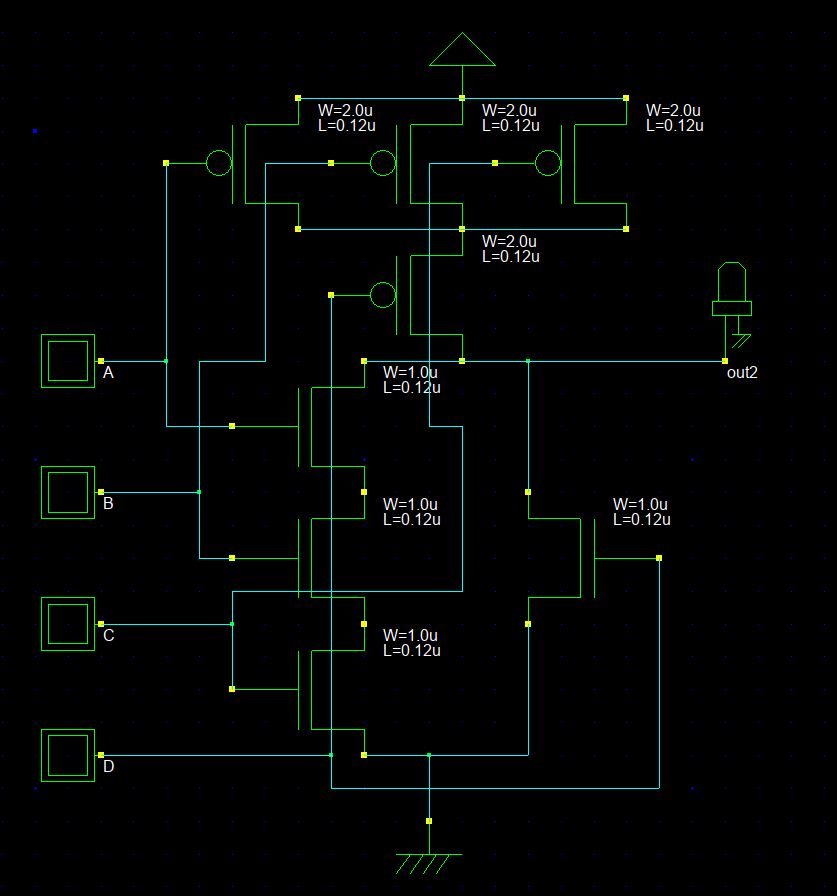
\includegraphics[width=0.5\textwidth]{Lab-02/output-1.png}
\caption{CMOS Schematic of $(ABC + D)'$}
\end{figure}

\subsection*{Timing Diagram}
\begin{figure}[!h]
\centering
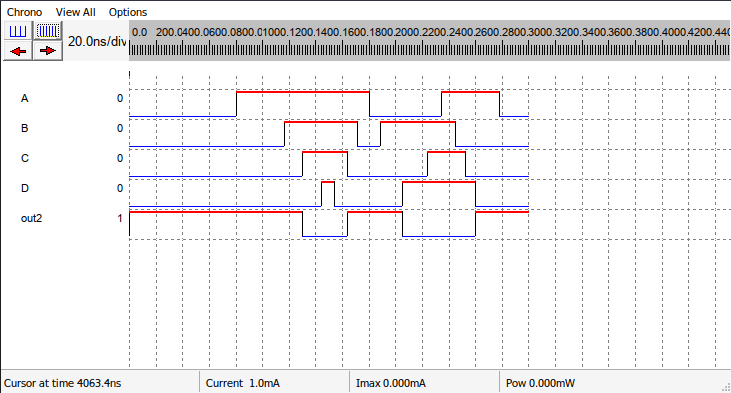
\includegraphics[width=0.7\textwidth]{Lab-02/timing-1.png}
\caption{Timing Diagram of $(ABC + D)'$}
\end{figure}
  
The timing diagram shows that the output remains HIGH except when all inputs A, B, and C are HIGH or when input D is HIGH.

\subsection*{Observation}
The simulation confirms that the output goes LOW when either $ABC=1$ or $D=1$. This matches the expected inverted logic behavior.

% =====================================================
\section{Function 2: $((AB + CD)E)'$}

\subsection*{Boolean Function}
\[
Y = ((AB + CD)E)'
\]

\subsection*{Truth Table}
\begin{center}
\begin{tabular}{|c|c|c|c|c|c|}
\hline
A & B & C & D & E & Y \\ \hline
0 & X & X & X & X & 1 \\
1 & 1 & X & X & 1 & 0 \\
0 & X & 1 & 1 & 1 & 0 \\ 
1 & X & X & X & 1 & 1 \\ \hline
\end{tabular}
\end{center}

\subsection*{Schematic Image}
\begin{figure}[!h]
\centering
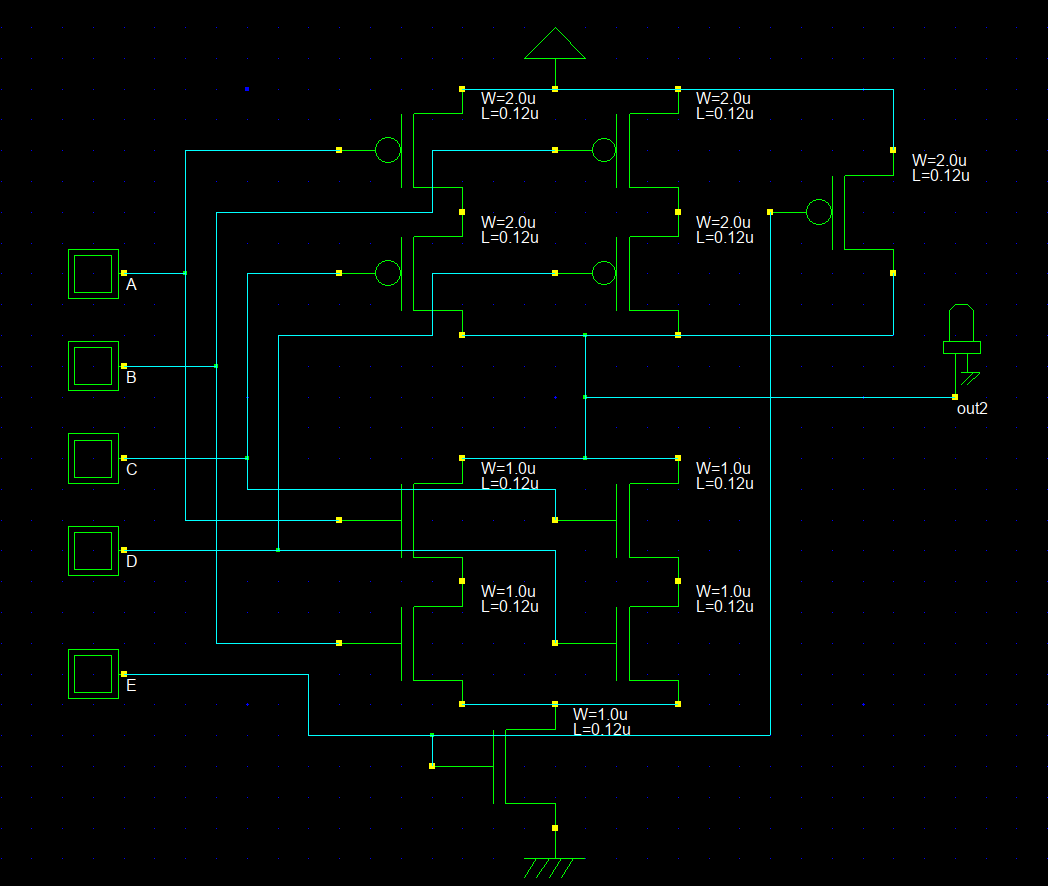
\includegraphics[width=0.9\textwidth]{Lab-02/output-2.png}
\caption{CMOS Schematic of $((AB+CD)E)'$}
\end{figure}
\newpage
\subsection*{Timing Diagram}
\begin{figure}[!h]
\centering
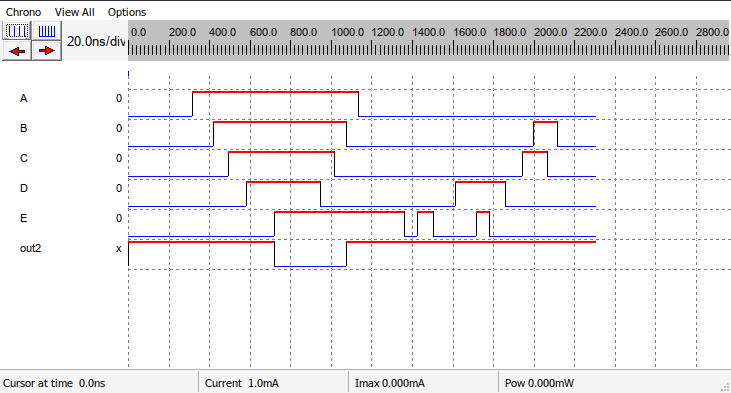
\includegraphics[width=0.9\textwidth]{Lab-02/timing-2.png}
\caption{Timing Diagram of $((AB+CD)E)'$}
\end{figure}

 
The output transitions LOW only when E is HIGH and either AB or CD is satisfied.

\subsection*{Observation}
The circuit output follows the complemented logic, validating correct CMOS pull-up and pull-down network operation.


% =====================================================
\section{Function 3: $((AB + C)(A + B))'$}

\subsection*{Boolean Function}
\[
Y = ((AB + C)(A + B))'
\]

\subsection*{Truth Table}
\begin{center}
\begin{tabular}{|c|c|c|c|}
\hline
A & B & C & Y \\ \hline
0 & 0 & 0 & 1 \\
0 & 1 & 0 & 1 \\
1 & 0 & 0 & 1 \\
1 & 1 & 0 & 0 \\
1 & 0 & 1 & 0 \\ 
1 & 1 & 1 & 0 \\ \hline
\end{tabular}
\end{center}
\newpage
\subsection*{Schematic Image}
\begin{figure}[!h]
\centering
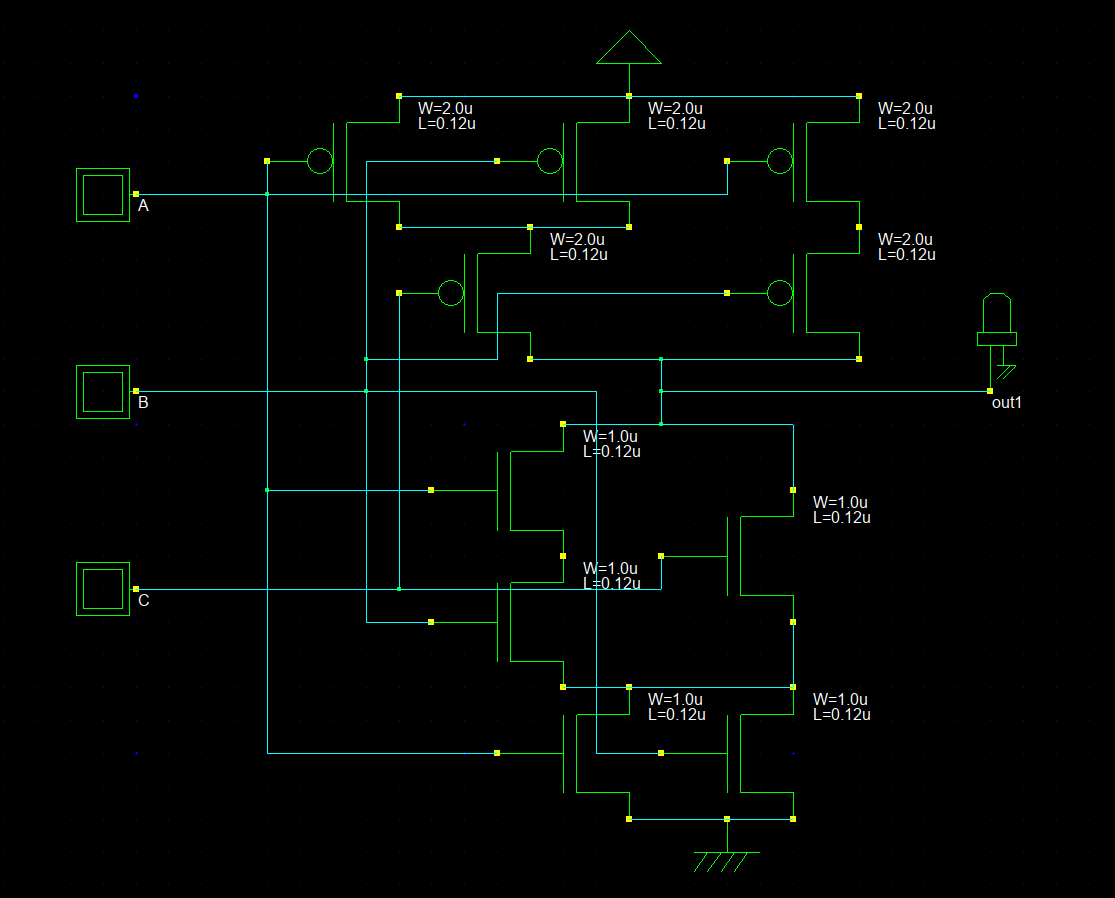
\includegraphics[width=0.8\textwidth]{Lab-02/output-3.png}
\caption{CMOS Schematic of $((AB + C)(A + B))'$}
\end{figure}

\subsection*{Timing Diagram}
\begin{figure}[!h]
\centering
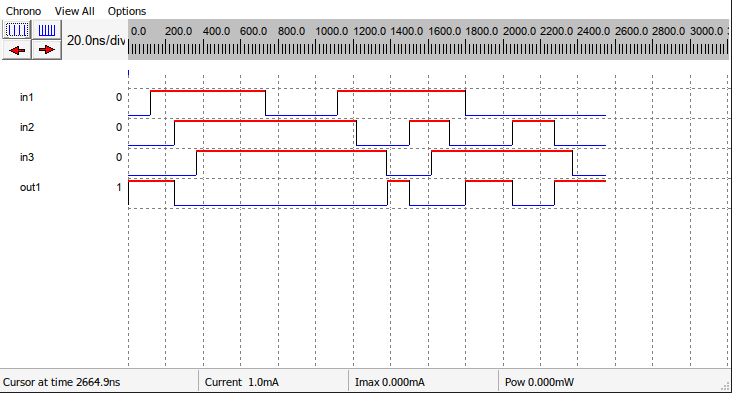
\includegraphics[width=0.8\textwidth]{Lab-02/timing-3.png}
\caption{Timing Diagram of $((AB + C)(A + B))'$}
\end{figure}

 
The output remains HIGH only when the AND of the two expressions is false.

\subsection*{Observation}
Simulation results matched the inverted product-of-sums logic expression.


% =====================================================
\section{Function 4: $(A + B + C)D$}

\subsection*{Boolean Function}
\[
Y = (A + B + C)D
\]

\subsection*{Truth Table}
\begin{center}
\begin{tabular}{|c|c|c|c|c|}
\hline
A & B & C & D & Y \\ \hline
X & X & X & 0 & 0 \\
1 & X & X & 1 & 1 \\
0 & 1 & X & 1 & 1 \\
0 & 0 & 1 & 1 & 1 \\
0 & 0 & 0 & 1 & 0 \\ \hline
\end{tabular}
\end{center}

\subsection*{Schematic Image}
\begin{figure}[!h]
\centering
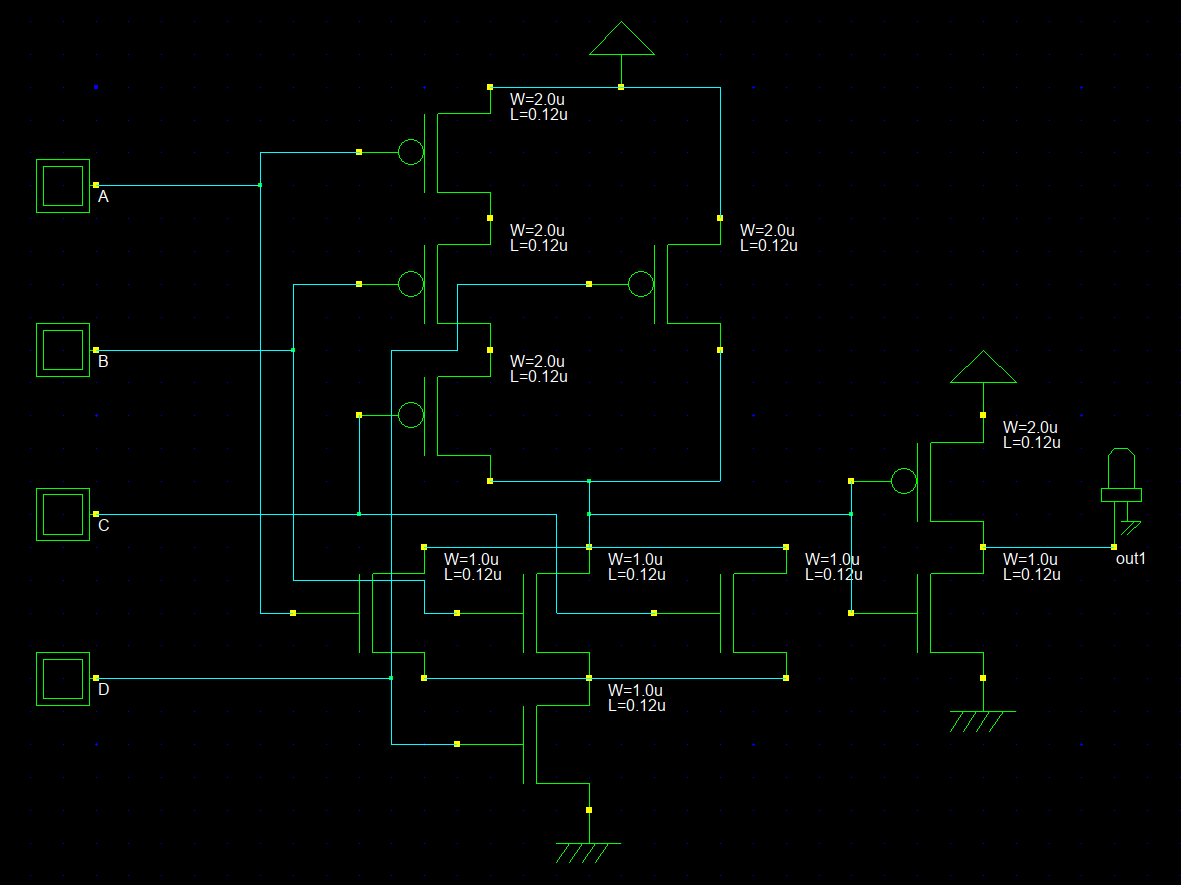
\includegraphics[width=0.9\textwidth]{Lab-02/output-4.png}
\caption{CMOS Schematic of $(A+B+C)D$}
\end{figure}
\newpage
\subsection*{Timing Diagram}
\begin{figure}[!h]
\centering
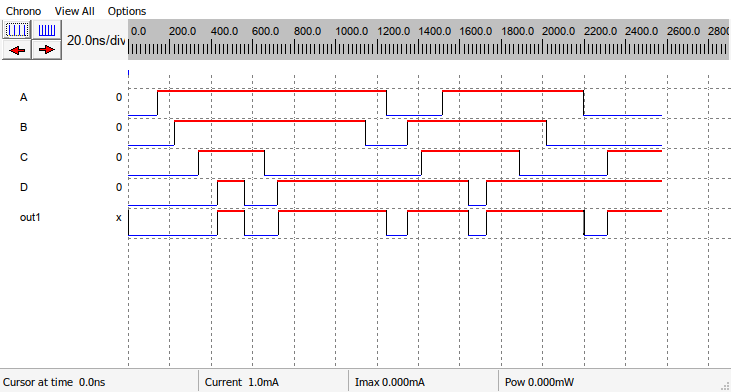
\includegraphics[width=0.9\textwidth]{Lab-02/timing-4.png}
\caption{Timing Diagram of $(A+B+C)D$}
\end{figure}
 
The output is HIGH only when D is HIGH and at least one of A, B, or C is HIGH.

\subsection*{Observation}
The simulation confirms correct AND–OR logic behavior.


% =====================================================
\section{Function 5: $((A + B)CD)'$}

\subsection*{Boolean Function}
\[
Y = ((A + B)CD)'
\]

\subsection*{Truth Table}
\begin{center}
\begin{tabular}{|c|c|c|c|c|}
\hline
A & B & C & D & Y \\ \hline
X & X & X & 0 & 1 \\
0 & 0 & 1 & 1 & 1 \\
1 & X & 1 & 1 & 0 \\
X & 1 & 1 & 1 & 0 \\ \hline
\end{tabular}
\end{center}
\newpage
\subsection*{Schematic Image}
\begin{figure}[!h]
\centering
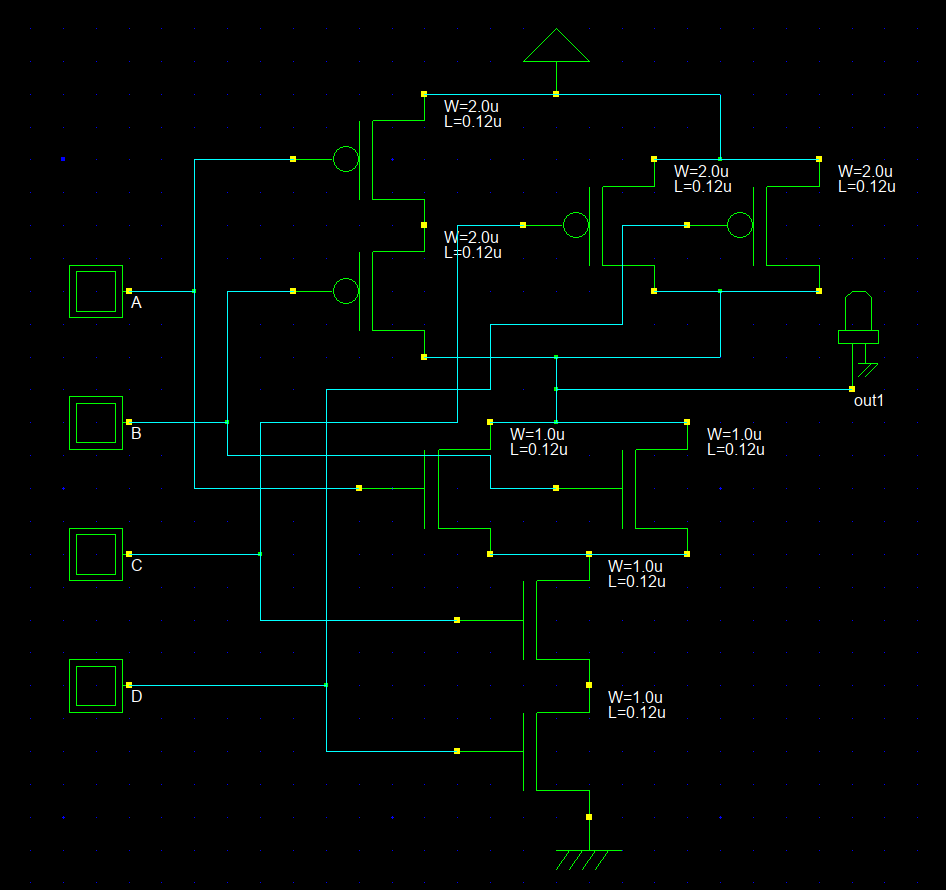
\includegraphics[width=0.6\textwidth]{Lab-02/output-5.png}
\caption{CMOS Schematic of $((A+B)CD)'$}
\end{figure}

\subsection*{Timing Diagram}
\begin{figure}[!h]
\centering
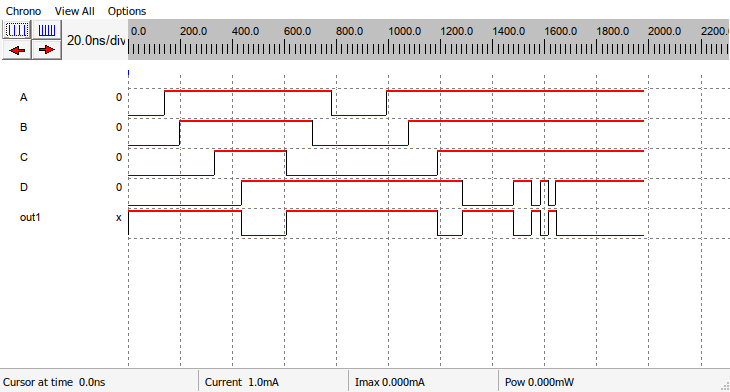
\includegraphics[width=0.8\textwidth]{Lab-02/timing-5.png}
\caption{Timing Diagram of $((A+B)CD)'$}
\end{figure}

\subsection*{Observation} 
The output goes LOW only when C and D are HIGH and either A or B is HIGH.
Simulation results confirm correct inverted AND–OR CMOS implementation.

% =====================================================






\chapter{Adder Circuits}
\lhead{Lab-03: Adder Circuits}
<Lab 3 Start here>




\chapter{Flip-Flop Circuits}
\lhead{Lab-04: Flip-Flop Circuits}
<Lab 4 Start here>




\chapter{Stick Diagram in MICROWIND2}
\lhead{Lab-05: Stick Diagram in MICROWIND2}
<Lab 5 Start here>




\chapter{Stick Diagram of XOR function}
\lhead{Lab-06: Stick Diagram of XOR function}
<Lab 6 Start here>





\end{document}